% !TeX document-id = {63e2cb4c-39e5-4fe5-ae31-d450d2286238}
% !TeX TXS-program:compile = txs:///pdflatex/[--shell-escape]
\documentclass[11pt,a4paper]{exam}
\printanswers % pour imprimer les réponses (corrigé)
%\noprintanswers % Pour ne pas imprimer les réponses (énoncé)
\addpoints % Pour compter les points
\usepackage[utf8]{inputenc}
\usepackage{minted}

\usepackage{algorithm} % pour faire du pseudo-code
\usepackage{algorithmicx} % pour faire du pseudo-code
\usepackage{algpseudocode} % pour faire du pseudo-code

% Traduction des commandes en pseudo-code
\renewcommand{\algorithmicfor}{\textbf{pour}}
\renewcommand{\algorithmicif}{\textbf{si}}
\renewcommand{\algorithmicthen}{\textbf{alors}}
\renewcommand{\algorithmicelse}{\textbf{sinon}}
\renewcommand{\algorithmicfunction}{\textbf{fonction}}
\renewcommand{\algorithmicforall}{\textbf{pour tout}}
\renewcommand{\algorithmicdo}{\textbf{faire}}
\renewcommand{\algorithmicwhile}{\textbf{tant que}}
\renewcommand{\algorithmicend}{\textbf{fin}}
\renewcommand{\algorithmicreturn}{\textbf{retourner}}
\renewcommand{\algorithmicrequire}{\textbf{Entrée:}}
\renewcommand{\algorithmicensure}{\textbf{Sortie:}} % Détournement du Ensure, mais ce n'est pas très grave...

\usepackage{geometry}
\usepackage{amsmath,amssymb}
\usepackage{multicol}
\usepackage{graphicx}
\usepackage{setspace}
\usepackage{dashundergaps}
%\usepackage[monochrome]{xcolor} % Permet de tout mettre en N&B strict
\usepackage{xcolor}
%\selectcolormodel{gray} % Permet de tout mettre en niveaux de gris
\geometry{left=0.8cm, right=0.8cm, top=2cm, bottom=1cm} % Définition des marges du doc

% Affichage propre des commandes shell
\usepackage{listings} % Pour l'affichage de code
% Configuration de l'affichage des listings
\lstset{
	language=bash, % Spécifie le langage
	basicstyle=\ttfamily\small, % Style de base
	keywordstyle=\color{blue}, % Style des mots-clés
	stringstyle=\color{red}, % Style des chaînes
	commentstyle=\color{green}, % Style des commentaires
	morecomment=[l][\color{magenta}]{\#}, % Couleur des commentaires de ligne
	frame=single, % Ajoute un cadre autour du code
	rulecolor=\color{black}, % Couleur du cadre
	tabsize=4, % Taille des tabulations
	numbers=left, % Place les numéros de ligne à gauche
	numberstyle=\tiny\color{gray}, % Style des numéros de ligne
	breaklines=true, % Permet le retour à la ligne automatique
	postbreak=\mbox{\textcolor{red}{$\hookrightarrow$}\space}, % Indique un retour à la ligne dans le code
	showstringspaces=false % N'affiche pas les espaces dans les chaînes
}

% Lettres de QCM
\usepackage{enumitem}
\newenvironment{QCM}
{\begin{enumerate}[label=\Alph*.]}
	{\end{enumerate}}


%\newcommand{\class}{1\textsuperscript{ère} Spé. NSI Gr. 2\textsubscript{A}}
\newcommand{\class}{1\textsuperscript{ère} Spé. NSI Gr. 2}
\newcommand{\examnum}{Contrôle \#5}
\newcommand{\examdate}{24/05/2024}
\newcommand{\timelimit}{1 Heure}
\newcommand{\lycee}{Lycée Fustel de Coulanges}

\pagestyle{head}
\firstpageheader{}{}{}
\runningheader{\class}{\examnum\ - Page \thepage\ / \numpages}{\examdate}
\runningheadrule


\begin{document}
% Espace d'en-tête
    \noindent
    \begin{spacing}{1}
        \noindent
        \begin{tabular*}{\textwidth}{l @{\extracolsep{\fill}} l @{\extracolsep{6pt}} l}
            \textbf{\class} & \textbf{\examnum, \examdate}&\\
            \textbf{\lycee} &\textbf{Durée: \timelimit} &\\
        \end{tabular*}\\
    \end{spacing}

    \noindent
    \vspace{10pt}
    \hrule
    \vspace{5pt} 
    \noindent
    \\
    Ce contrôle comporte \numquestions\ questions; le nombre maximal possible de points est de \numpoints. 
    Les réponses sont à porter sur une copie \uline{comportant votre nom}.
    Il n'est pas nécessaire de répondre aux questions dans l'ordre \textemdash\ commencez par celles où vous vous sentez le plus à l'aise.\\
    Les calculatrices ne sont \uline{pas} autorisées.\\
    \noindent
    \hrule
    \vspace{15pt} 

    \begin{questions} % DEBUT DE L'EXAMEN
		\begin{spacing}{1}
    
		\question \textit{Questions de cours}
		\begin{parts}
			\part[3]{QCM -- les réponses sont à porter sur votre copie; il n'est pas nécessaire de justifier vos réponses; une seule réponse par question.}
			\begin{subparts}
			
				\subpart Quel est le rôle principal d'un système d'exploitation?
				\begin{QCM}
					\item Compiler les programmes.
					\item Gérer les ressources matérielles et logicielles de l'ordinateur.
					\item Créer des documents.
					\item Réaliser des calculs mathématiques.
				\end{QCM}
				\begin{solution}
					B. Gérer les ressources matérielles et logicielles de l'ordinateur.
				\end{solution}

				\subpart Parmi les éléments suivants lequel n'est pas une tâche du système d'exploitation?
				\begin{QCM}
					\item Gestion de la mémoire.
					\item Gestion des fichiers
					\item Traitement de texte.
					\item Gestion des périphériques.
				\end{QCM}
				\begin{solution}
					C. Traitement de texte.
				\end{solution}
				
				\subpart Quel est le rôle d'un routeur dans un réseau informatique?
				\begin{QCM}
					\item Connecter des ordinateurs à un réseau local.
					\item Traduire les adresses web en adresses IP.
					\item Acheminer les paquets de données entre différents réseaux.
					\item  Stocker les données des utilisateurs.
				\end{QCM}
				\begin{solution}
					C. Acheminer les paquets de données entre différents réseaux.
				\end{solution}
				
				\subpart Quelle composante de l'architecture de von Neumann est responsable de l'exécution des instructions?
				\begin{QCM}
					\item Unité de contrôle.
					\item Mémoire.
					\item Unité de stockage.
					\item  Périphériques d'entrée/sortie.
				\end{QCM}
				\begin{solution}
					A. Unité de contrôle.
				\end{solution}
				
				\subpart Le langage assembleur est un type de:
				\begin{QCM}
					\item Langage de haut niveau.
					\item Langage de programmation visuel.
					\item Langage de bas niveau.
					\item  Langage de script.
				\end{QCM}
				\begin{solution}
					C. Langage de bas niveau.
				\end{solution}
				
				\subpart Quelle est la différence principale entre le langage machine et le langage assembleur ?
				\begin{QCM}
					\item Le langage machine utilise des instructions compréhensibles par les humains.
					\item Le langage assembleur utilise des instructions symboliques compréhensibles par les humains.
					\item Le langage assembleur est plus rapide à exécuter que le langage machine.
					\item  Le langage machine est plus facile à lire et à écrire que le langage assembleur.
				\end{QCM}
				\begin{solution}
					B. Le langage assembleur utilise des instructions symboliques compréhensibles par les humains.
				\end{solution}
				\end{subparts}
			
			\part[1] Lorsqu'on gère les droits qu'un utilisateur a sur un fichier dans un environnement Linux, on utilise les lettres "\texttt{r}", "\texttt{w}", et "\texttt{x}". Expliquez brièvement à quoi chacune correspond.
			\begin{solution}
				\begin{itemize}
					\item \texttt{r} (read) : Permet la lecture du fichier.
					\item \texttt{w} (write) : Permet la modification du fichier.
					\item \texttt{x} (execute) : Permet l’exécution du fichier s’il s’agit d’un programme ou d’un script.
				\end{itemize}
			\end{solution}

			\part[1] Dans le contexte des réseaux informatiques, qu’est-ce qu’un protocole? À quoi cela sert-il?
			\begin{solution}
				Tout ou partie des éléments suivants était attendu: un protocole est un ensemble de règles et de conventions définissant le format, la séquence et la gestion des erreurs des échanges de données sur un réseau. Il sert à assurer une communication cohérente et efficace entre les périphériques sur un réseau.
			\end{solution}
			
			\part[1] Qu'entend-on par l'expression "passerelle par défaut"? Que désigne-t-elle et à quoi sert-elle?
			\begin{solution}
				Tout ou partie des éléments suivants était attendu: la passerelle par défaut est l’adresse IP du routeur utilisée par un périphérique pour envoyer des paquets de données à des destinations hors de son réseau local. Elle sert de point de sortie pour les données à destination de réseaux distants --- internet notamment.
			\end{solution}
			
			\part[1] Listez deux différences entre une adresse MAC et une adresse IP.
			\begin{solution}
				Deux parmi les différences suivantes étaient attendues:
				\begin{itemize}
					\item Une adresse MAC est une adresse matérielle associée à une carte réseau, tandis qu’une adresse IP est une adresse logicielle attribuée à un périphérique sur un réseau.
					\item Les adresses MAC sont assignées par le fabricant de la carte réseau et sont généralement permanentes, tandis que les adresses IP sont attribuées dynamiquement par un protocole réseau et peuvent changer.
					\item Les adresses MAC fonctionnent au niveau de la couche réseau du modèle TCP/IP tandis que les adresses IP fonctionnent au niveau de la couche internet.
					\item Les adresses MAC sont codées sur 48 bits (6 octets), tandis que les adresses IPv4 sont codées sur 32 bits (4 octets) et les adresses IPv6 sur 128 bits (16 octets).
					\item Une adresse MAC est unique tandis qu'une adresse IP peut exister simultanément à l'intérieur de différents réseaux.
				\end{itemize}
			\end{solution}
			
			\part[1] Pourquoi utilise-t-on des registres en assembleur alors qu'on n'en parle pas en Python?
			\begin{solution}
				Les registres (espaces mémoire à l'intérieur du processeur, d'accès extrêmement rapide) en assembleur sont utilisés pour stocker des données temporaires et pour effectuer des opérations arithmétiques et logiques. Ils sont essentiels pour manipuler efficacement les données directement sur le processeur. En Python, les registres ne sont pas directement accessibles car le langage est de haut niveau et délègue donc la gestion de la mémoire au système d'exploitation.
			\end{solution}
		\end{parts}
		
		% (supprimée de la correction)
		%\pagebreak
		
		\question{\textit{Commandes shell}}
		
		Je me trouve dans le répertoire \texttt{/home/nsi} et j'exécute les commandes suivantes:
		\begin{lstlisting}
mkdir controle
cd controle
mkdir src
mkdir doc
cd src
touch main.py
touch utils.py
cd ../doc
touch README.txt
cd ../../..
pwd
		\end{lstlisting}
		
		\begin{parts}
			\part[1] Dessinez l’arborescence créée par ces commandes.
			\begin{solution}
				Une manière possible de représenter cette arborescence était la suivante:
				\begin{figure}[H]
					\centering
					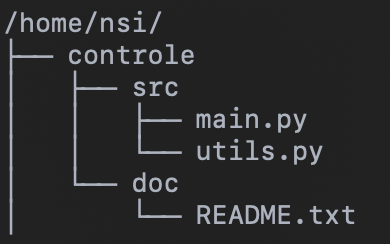
\includegraphics[width=0.3\textwidth]{Arbo.png}
				\end{figure}
			\end{solution}
			\part[1] Quel sera le retour de la dernière commande (qu’est-ce qui va s’afficher dans la console à l'exécution de "\texttt{pwd}")?
			\begin{solution}
				On est, depuis le point de départ \texttt{/home/nsi/} "descendus" deux fois dans les lignes précédentes (d'abord dans \texttt{controle} puis dans \texttt{doc}) puis, dans la ligne juste au-dessus, on est "remontés" de trois niveaux ("\texttt{../../..}"). On est donc un cran au-dessus de notre point de départ et le retour du \texttt{pwd} sera:
				
				\texttt{/home}
			\end{solution}
			\part[1] En une, deux, ou trois commandes successives à la suite des précédentes, faites afficher dans la console le contenu du fichier README.txt.
			\begin{solution}
				En deux commandes (je vous laisse deviner ce que cela donne en une ou en trois), cela donne:
				\begin{lstlisting}
cd controle/doc
cat README.txt
				\end{lstlisting}
				
			\end{solution}
			\part[1] On souhaite que le fichier \texttt{utils.py} soit: lisible, modifiable, et exécutable uniquement par le propriétaire --- et qu'il n'y ait aucun droit pour les autres. Quelle commande \texttt{chmod} doit-on utiliser pour cela?
			\begin{solution}
				On veut tous les droits pour le propriétaire, donc \texttt{r}, \texttt{w} et \texttt{x} à 1, donc au total: $(111)_2 = 7_{10}$; on ne veut aucun droit pour les autres, donc 0 dans les deux cas:
				
				\texttt{chmod 700 /home/nsi/controle/src/utils.py}
			\end{solution}
			\part[1] On souhaite que le fichier \texttt{main.py} soit: exécutable uniquement par le propriétaire; modifiable par le propriétaire et par le groupe; et lisible par tout le monde (propriétaire, groupe, et autres). Quelle commande chmod doit-on utiliser pour cela?
			\begin{solution}
				On veut tous les droits pour le propriétaire, donc 7 (voir ci-dessus); pour le groupe on veut les droits \texttt{r} et \texttt{w} à 1, donc $(110)_2 = 6_{10}$; et pour les autres on ne veut que \texttt{r} à 1, donc $(100)_2 = 4_{10}$. Donc:
				
				\texttt{chmod 764 /home/nsi/controle/src/main.py}
			\end{solution}
		\end{parts}

        \question[2]{\textit{Masques de sous-réseau}}
       	
       	Soit l'adresse IP et masque de sous-réseau (en notation CIDR) \texttt{192.168.1.50/26}. Combien d'adresses IP distinctes peuvent-elles exister dans ce réseau? Quelle est la première (avec la valeur la plus faible)? Quelle est la dernière?
        \begin{solution}
        	En notation CIDR \texttt{192.168.1.50/26} signifie que les 26 premiers bits de l'adresse IP correspondent à l'adresse réseau. Étant donné qu'une adresse IP est codée sur 4 octets, donc 32 bits, cela signifie qu'il reste 6 bits pour l'adresse de l'hôte, pour un total de $2^6 = 64$ adresses possibles.
        	
        	Pour déterminer la Appliquons d'abord le "ET" du masque de sous-réseau pour déterminer l'adresse exacte du réseau. Le masque de sous réseau est constitué des trois premiers octets tous à 1 (24 bits) puis de deux bits à 1 et enfin des six derniers à 0. L'adresse IP, elle, est donc 192.168.1 puis 50 que nous convertissons en binaire: $50 = 32 + 16 + 2 = 2^5 + 2^4 + 2^1 = (110010)_2$
        	\[
        	\begin{array}{r *{9}{@{\;}r}}
        		 & 192.168.1. & 0 & 0 & 1 & 1 & 0 & 0 & 1 & 0\\
        		\textbf{ET} & 255.255.255. & 1 & 1 & 0 & 0 & 0 & 0 & 0 & 0 \\
        		\cline{1-10}
        		& 192.168.1. & 0 & 0 & 0 & 0 & 0 & 0 & 0 & 0\\
        	\end{array}
        	\]
        	La première adresse est ainsi celle qui a les 6 derniers bits à 0 et la dernière celle qui a les 6 derniers bits à 1, soit, une fois converti en décimal: \texttt{192.168.1.0} et \texttt{192.168.1.63} (pour un total qui fait donc bien les 64 que l'on a calculés plus haut).
        	
        	Remarque: strictement parlant, ces deux adresses sont, respectivement, l'adresse du réseau lui-même et l'adresse dite "de broadcast", c'est-à-dire l'adresse utilisée pour envoyer simultanément un message à tous les périphériques connectés à ce réseau. Donc les adresses disponibles pour de "vrais" périphériques sont en fait celles allant de \texttt{192.168.1.1} à \texttt{192.168.1.62}.
        \end{solution}
		
		\question[2]{\textit{Masques de sous-réseau --- suite}}
		
		Soit l'adresse IP 192.168.10.5 et le masque de sous-réseau 255.255.255.240. Parmi les adresses IP suivantes, lesquelles appartiennent au même réseau que 192.168.10.5? \textbf{[ATTENTION: il est demandé le détail du calcul pour chacune des adresses -- une réponse sans justification ne rapportera aucun point]}
		\begin{itemize}
			\item \texttt{192.168.10.9}
			\item \texttt{192.168.10.14}
			\item \texttt{192.168.10.18}
			\item \texttt{192.168.10.3}
		\end{itemize}
		\begin{solution}
			Le masque de sous réseau étant constitué de trois 255 pour les trois premiers octets, toutes les adresses du réseau commenceront bien par 192.168.10. Pour ce qui est du dernier octet on va appliquer à chacune des adresses listées le "ET" du masque de sous-réseau pour pouvoir conclure. On commence par convertir 240 en binaire: $240 = 255 - 15 = 255 - 1 - 2 - 4 - 8 = 255 - 2^0 - 2^1 - 2^2 - 2^3 = (11110000)_2$.
			
			On applique le masque de sous-réseau aux 5 adresses (celle de base et les quatre de l'énoncé). On commence par convertir en binaire les valeurs du dernier octet de chacune d'entre elles:
			\begin{itemize}
				\item $5 = 4 + 1 = 2^2 + 2^0 = (101)_2$
				\item $9 = 8 + 1 = 2^3 + 2^0 = (1001)_2$
				\item $14 = 8 + 4 + 2 = 2^3 + 2^2 + 2^1 = (1110)_2$
				\item $18 = 16 + 2 = 2^4 + 2^1 = (10010)_2$
				\item $3 = 2 + 1 = 2^1 + 2^0 = (11)_2$
			\end{itemize}
			\[
			\begin{minipage}{0.3\textwidth}
				\center{5:}
				\[
				\begin{array}{r *{8}{@{\;}r}}
					& 0 & 0 & 0 & 0 & 0 & 1 & 0 & 1\\
					\textbf{ET} & 1 & 1 & 1 & 1 & 0 & 0 & 0 & 0 \\
					\cline{1-9}
					& 0 & 0 & 0 & 0 & 0 & 0 & 0 & 0\\
				\end{array}
				\]
			\end{minipage}
			\hfill
			\begin{minipage}{0.3\textwidth}
				\center{9:}
				\[
				\begin{array}{r *{8}{@{\;}r}}
					& 0 & 0 & 0 & 0 & 1 & 0 & 0 & 1\\
					\textbf{ET} & 1 & 1 & 1 & 1 & 0 & 0 & 0 & 0 \\
					\cline{1-9}
					& 0 & 0 & 0 & 0 & 0 & 0 & 0 & 0\\
				\end{array}
				\]
			\end{minipage}
			\hfill
			\begin{minipage}{0.3\textwidth}
				\center{14:}
				\[
				\begin{array}{r *{8}{@{\;}r}}
					& 0 & 0 & 0 & 0 & 1 & 1 & 1 & 0\\
					\textbf{ET} & 1 & 1 & 1 & 1 & 0 & 0 & 0 & 0 \\
					\cline{1-9}
					& 0 & 0 & 0 & 0 & 0 & 0 & 0 & 0\\
				\end{array}
				\]
			\end{minipage}
			\]
			\[
			\begin{minipage}{0.5\textwidth}
				\center{18:}
				\[
				\begin{array}{r *{8}{@{\;}r}}
					& 0 & 0 & 0 & 1 & 0 & 0 & 1 & 0\\
					\textbf{ET} & 1 & 1 & 1 & 1 & 0 & 0 & 0 & 0 \\
					\cline{1-9}
					& 0 & 0 & 0 & 1 & 0 & 0 & 0 & 0\\
				\end{array}
				\]
			\end{minipage}
			\hfill
			\begin{minipage}{0.5\textwidth}
				\center{3:}
				\[
				\begin{array}{r *{8}{@{\;}r}}
					& 0 & 0 & 0 & 0 & 0 & 0 & 1 & 1\\
					\textbf{ET} & 1 & 1 & 1 & 1 & 0 & 0 & 0 & 0 \\
					\cline{1-9}
					& 0 & 0 & 0 & 0 & 0 & 0 & 0 & 0\\
				\end{array}
				\]
			\end{minipage}
			\]
			On constate immédiatement que tous les résultats sont à 0 à l'exception de l'avant-dernier qui est à $00010000_2$. On peut donc en conclure que toutes les adresses listées font partie du même réseau à l'exception de \texttt{192.168.10.18}.
		\end{solution}
		
		\question[3]{\textit{Consultation d'une page web}}
		
		\textit{Lorsqu'un serveur web envoie des données à un navigateur, les données sont encapsulées dans des segments UDP à la couche transport, utilisant le port 80. Ces segments sont ensuite encapsulés dans des paquets TCP (couche internet), qui sont à leur tour encapsulés dans des trames Wi-Fi à la couche réseau. Chaque trame contient une adresse IP unique pour identifier les appareils. Le protocole TCP assure un transfert rapide des données sans vérifier leur intégrité. Finalement, les trames sont transmises sur le réseau via des ondes radio.}
		
		Le texte ci-dessus contient 6 erreurs: identifiez-en (au moins) 3 \uline{et donnez-en la correction}. \textit{(Si vous en identifiez plus, cela vous vaudra des points bonus -- 0,5 point par erreur supplémentaire.)}
		\begin{solution}
			Voici le texte, ré-écrit avec en gras les 6 erreurs corrigées:
			
			\textit{Lorsqu’un serveur web envoie des données à un navigateur, les données sont encapsulées dans des segments \textbf{TCP} à la couche transport, utilisant le port 80. Ces segments sont ensuite encapsulés dans des paquets \textbf{IP} (couche Internet), qui sont à leur tour encapsulés dans des trames \textbf{Ethernet} à la couche réseau. Chaque trame contient une adresse \textbf{MAC} unique pour identifier les appareils. Le protocole TCP assure un transfert \textbf{fiable des données en vérifiant leur intégrité}. Finalement, les trames sont transmises sur le réseau via, principalement, \textbf{des câbles Ethernet}.}
		\end{solution}
        \end{spacing}
    \end{questions}
\end{document}

% Séparation entre questions normales et questions bonus (N/A ici)
\vspace{1.5\baselineskip} 
\hrule
\vspace{1.5\baselineskip} 

% For future use: ET de masque de sous-réseau:
Pour déterminer la Appliquons d'abord le "ET" du masque de sous-réseau pour déterminer l'adresse exacte du réseau. Le masque de sous réseau est constitué des trois premiers octets tous à 1 (24 bits) puis de deux bits à 1 et enfin des six derniers à 0. L'adresse IP, elle, est donc 192.168.1 puis 50 que nous convertissons en binaire: $50 = 32 + 16 + 2 = 2^5 + 2^4 + 2^1 = (110010)_2$
\[
\begin{array}{r *{9}{@{\;}r}}
	& 192.168.1. & 0 & 0 & 1 & 1 & 0 & 0 & 1 & 0\\
	\textbf{ET} & 255.255.255. & 1 & 1 & 0 & 0 & 0 & 0 & 0 & 0 \\
	\cline{1-10}
	& 192.168.1. & 0 & 0 & 0 & 0 & 0 & 0 & 0 & 0\\
\end{array}
\]